

This appendix includes examples showing the use of different functionalities
implemented in the package. These \textit{Python notebooks} are available
together with the 
\href{https://fda.readthedocs.io/en/latest/auto_examples/}{online} documentation.

The examples included in this annex are:

\begin{enumerate}
\item Interpolation
\item Extrapolation
\item Composition
\item Shift registration
\item Landmark shift
\item Landmark registration
\item Pairwise alignment
\item Elastic registration
\item K-nearest neighbors classification
\item Radius-nearest neighbors classification
\item Neighbors scalar regressions

\end{enumerate}


%\section{Interpolation\label{EX:INTERPOLATION}}

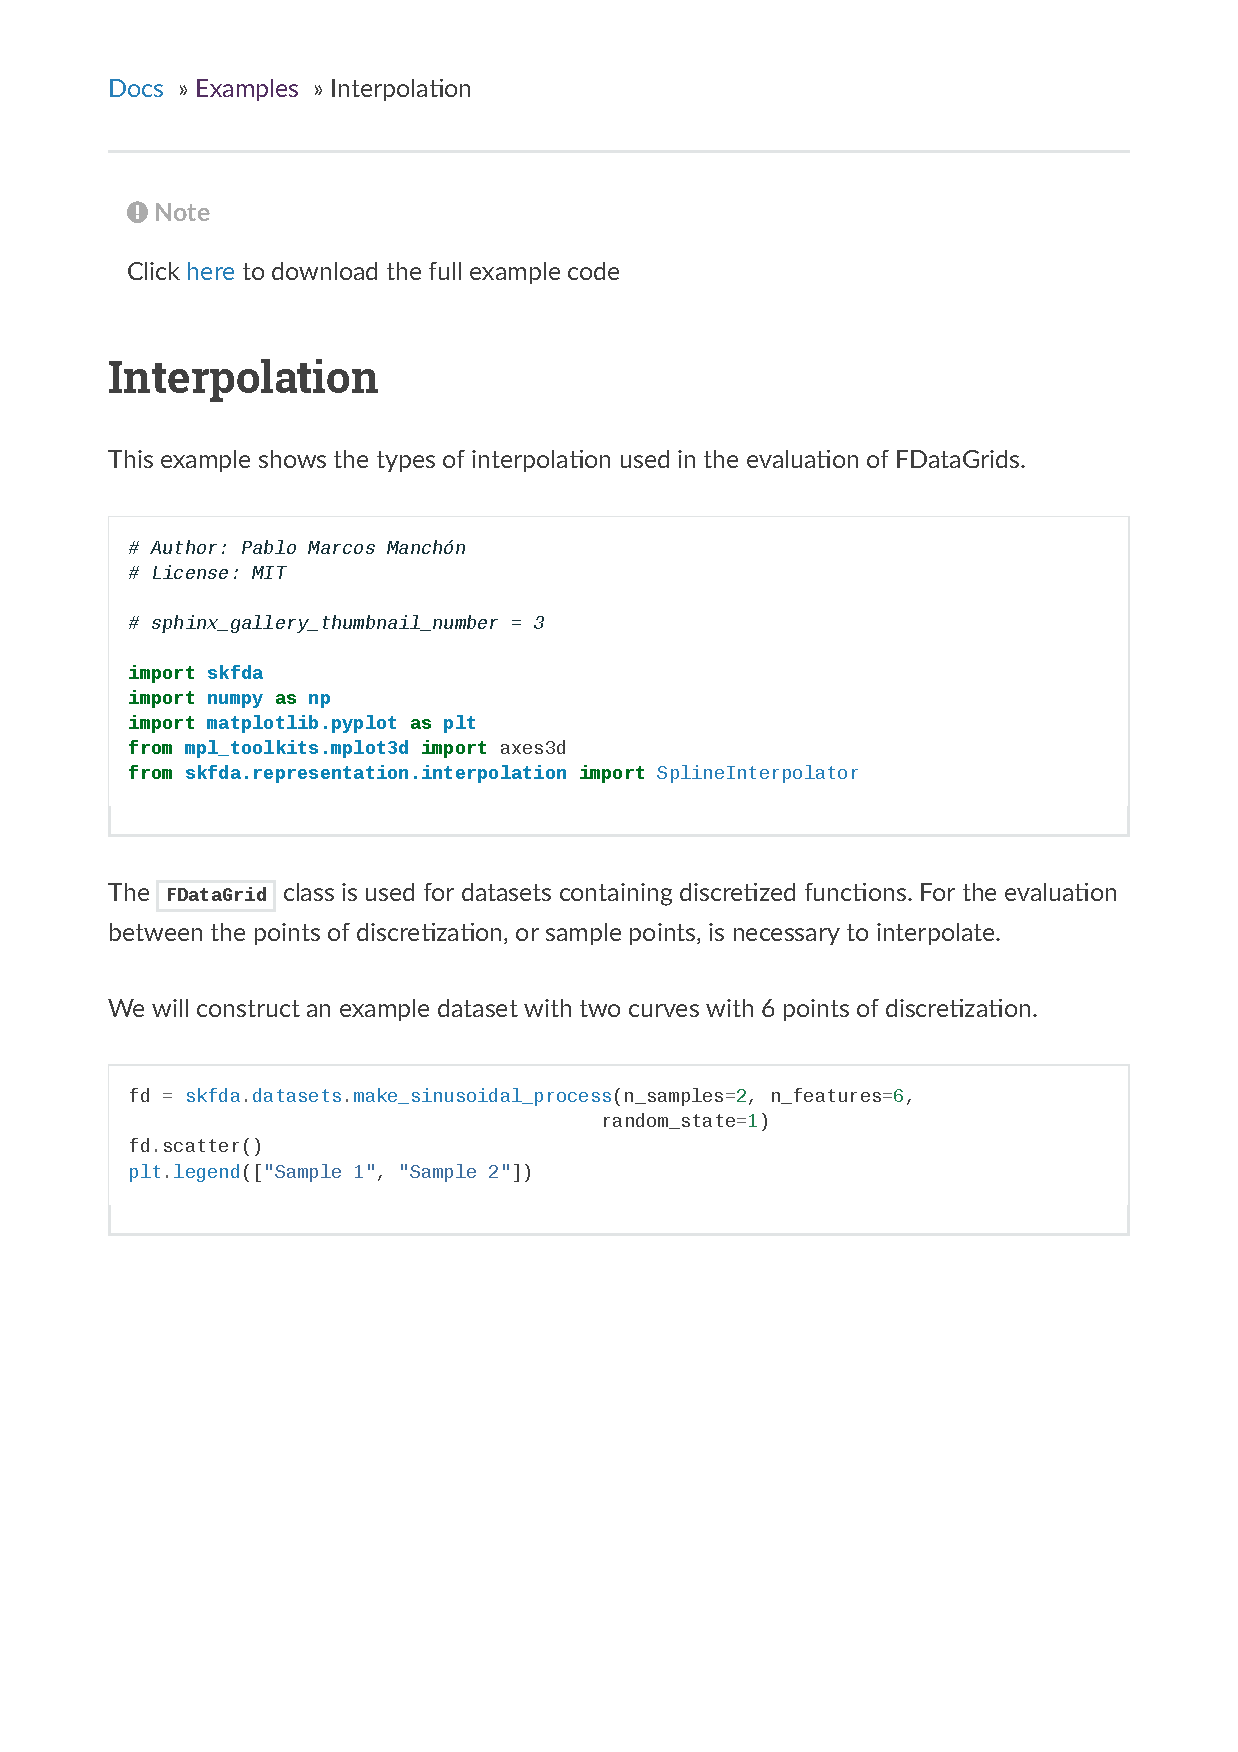
\includepdf[pages=-, nup=2x2]{notebooks-pdf/Interpolation}

%\section{Extrapolation\label{EX:EXTRAPOLATION}}

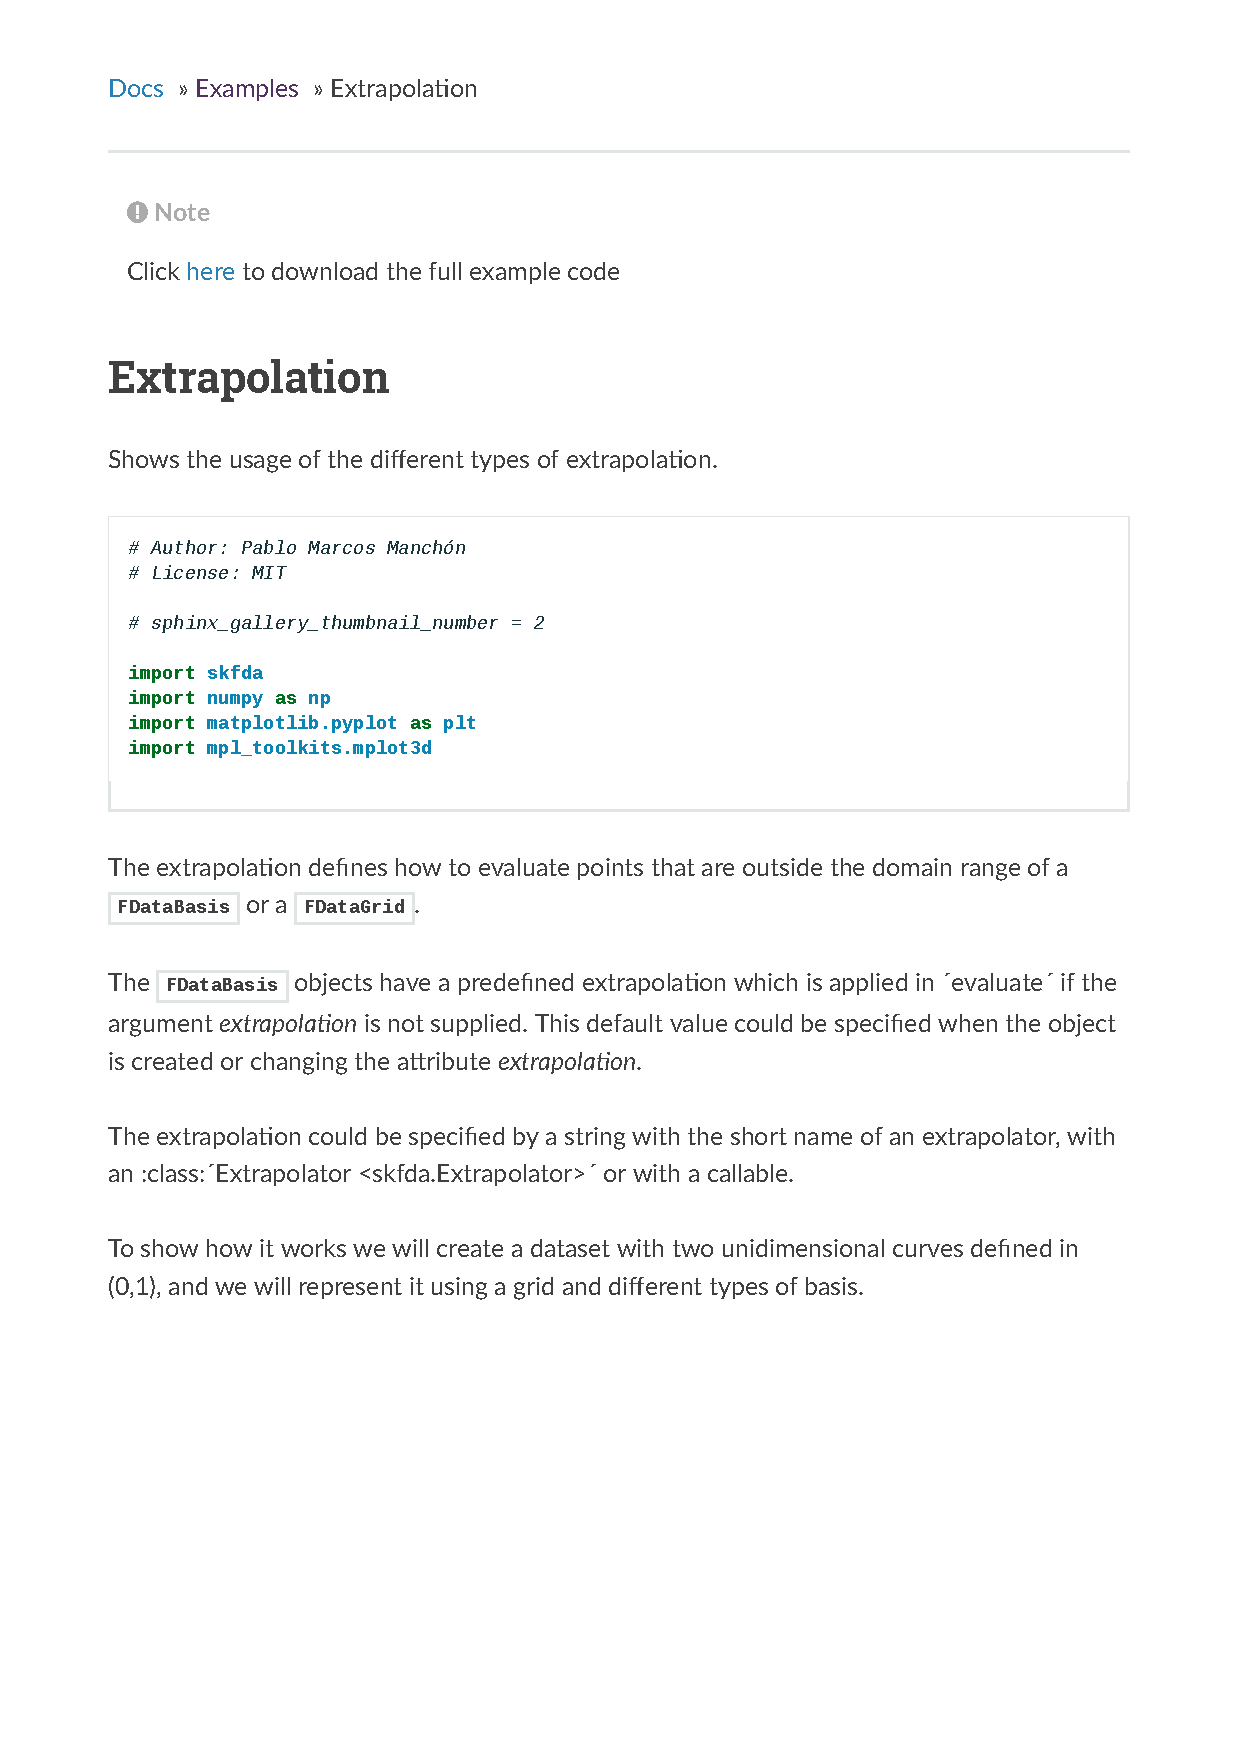
\includepdf[pages=-, nup=2x2]{notebooks-pdf/Extrapolation}

%\section{Composition\label{EX:COMPOSITION}}

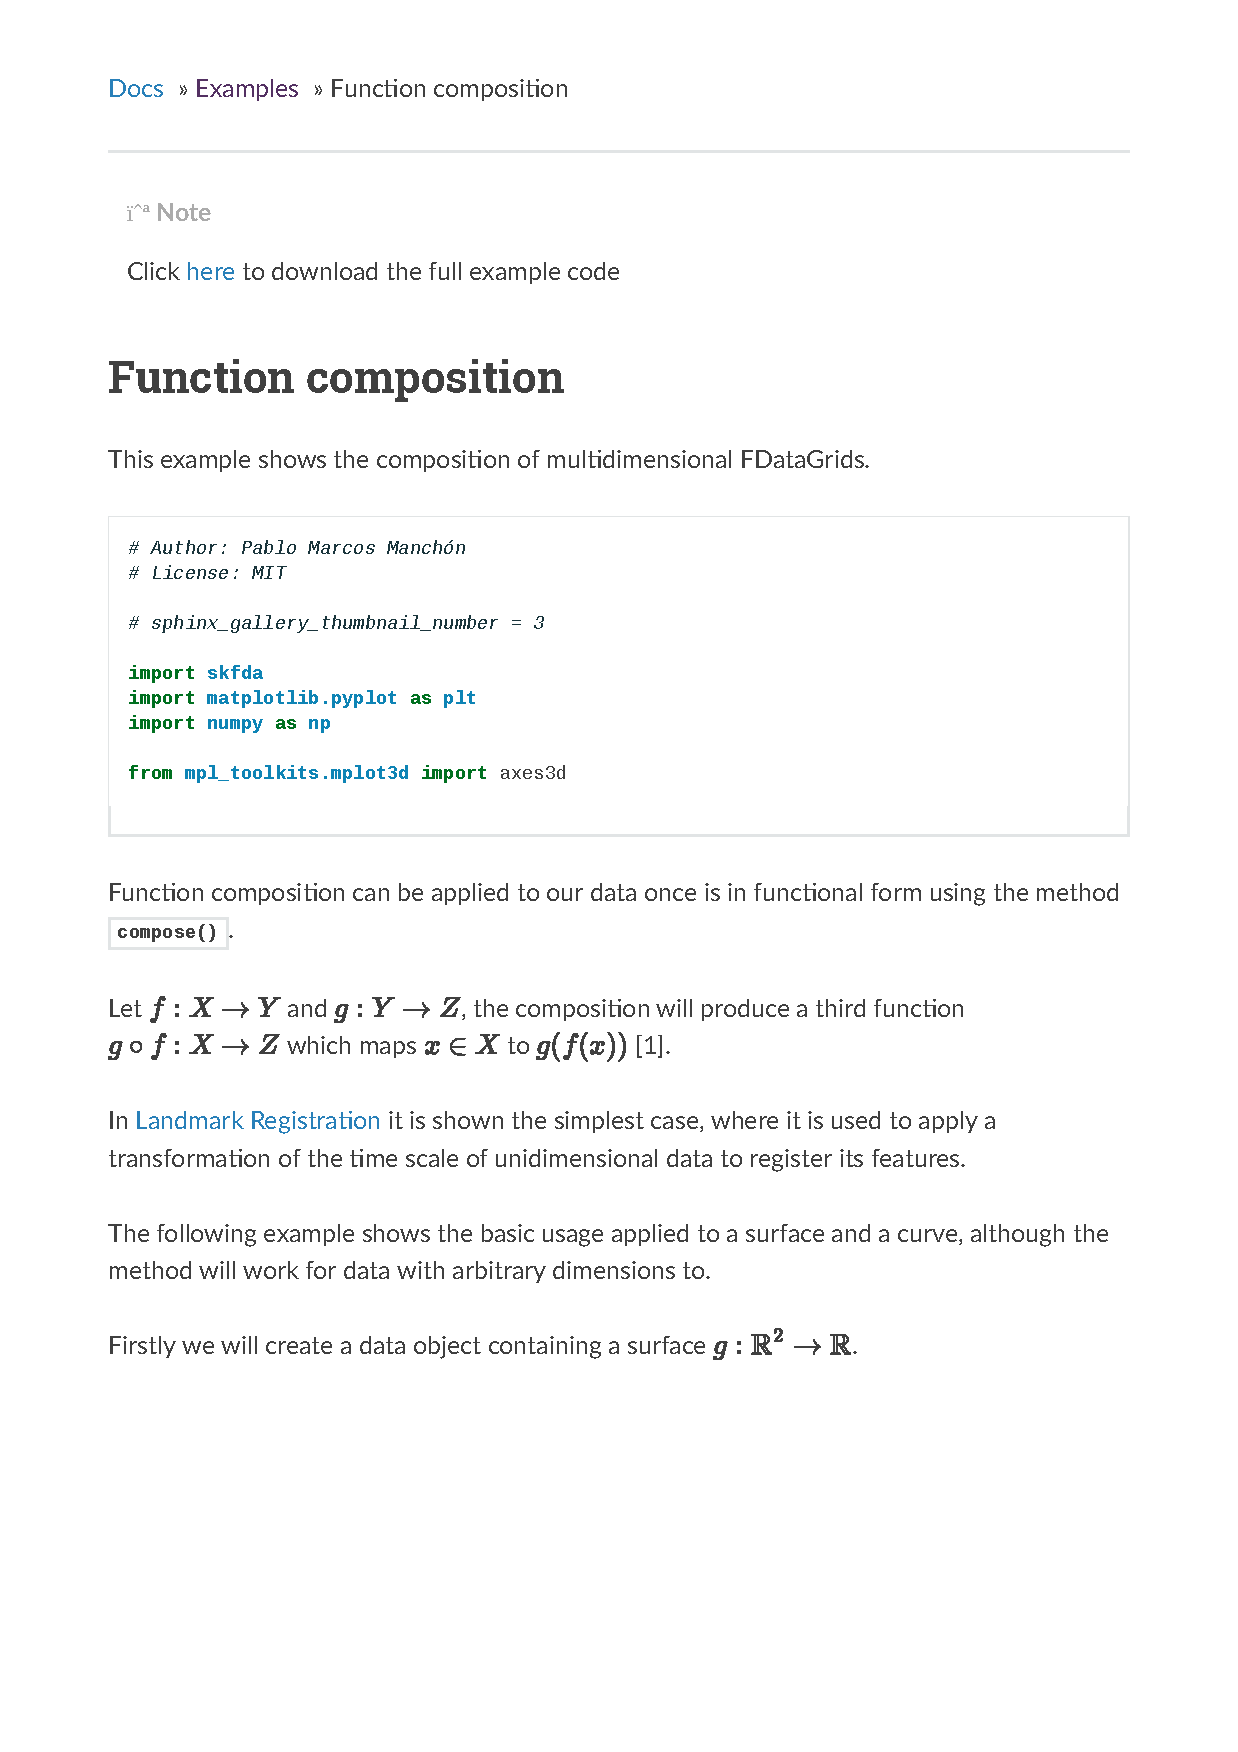
\includepdf[pages=-, nup=2x2]{notebooks-pdf/Composition}

%\section{Shift registration\label{EX:SHIFT}}

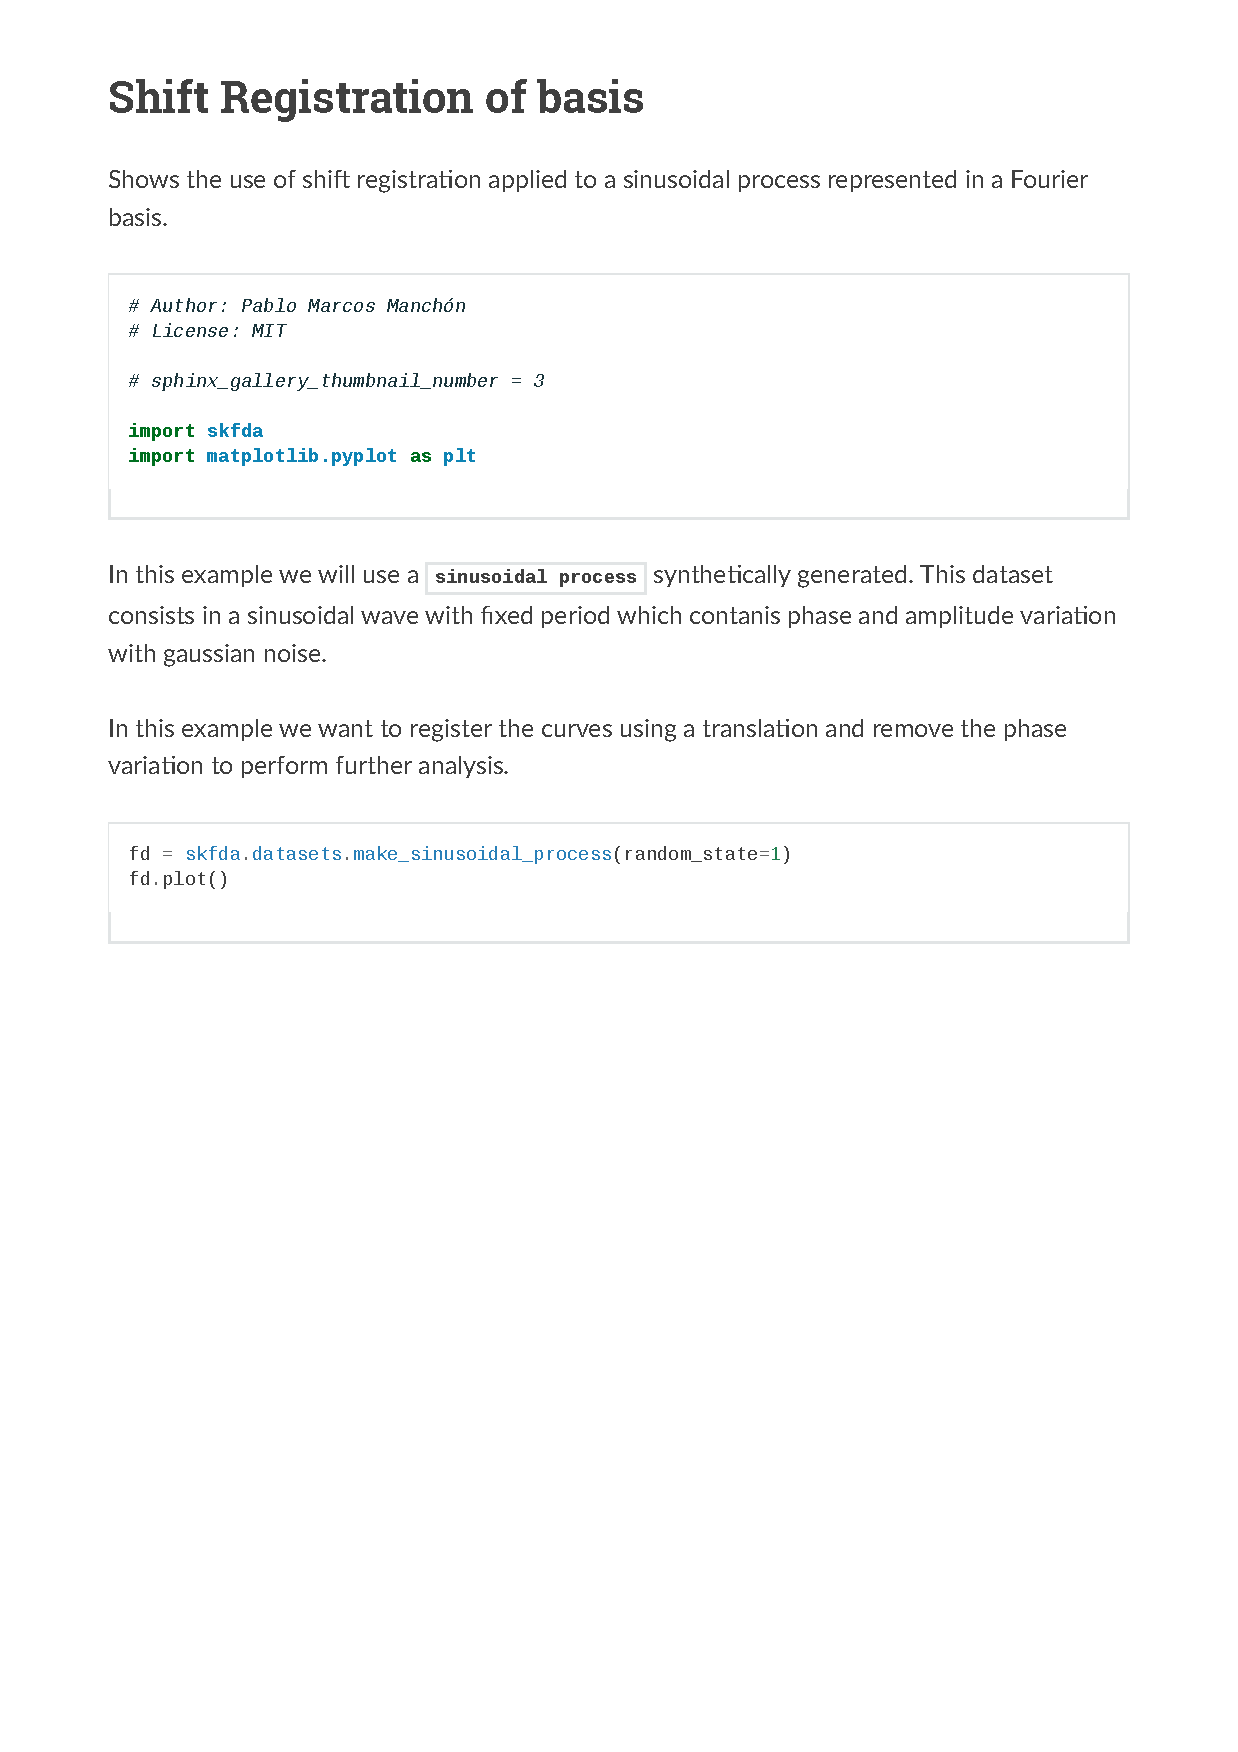
\includepdf[pages=-, nup=2x2]{notebooks-pdf/Shift-registration}

%\section{Landmark shift\label{EX:LANDSHIFT}}

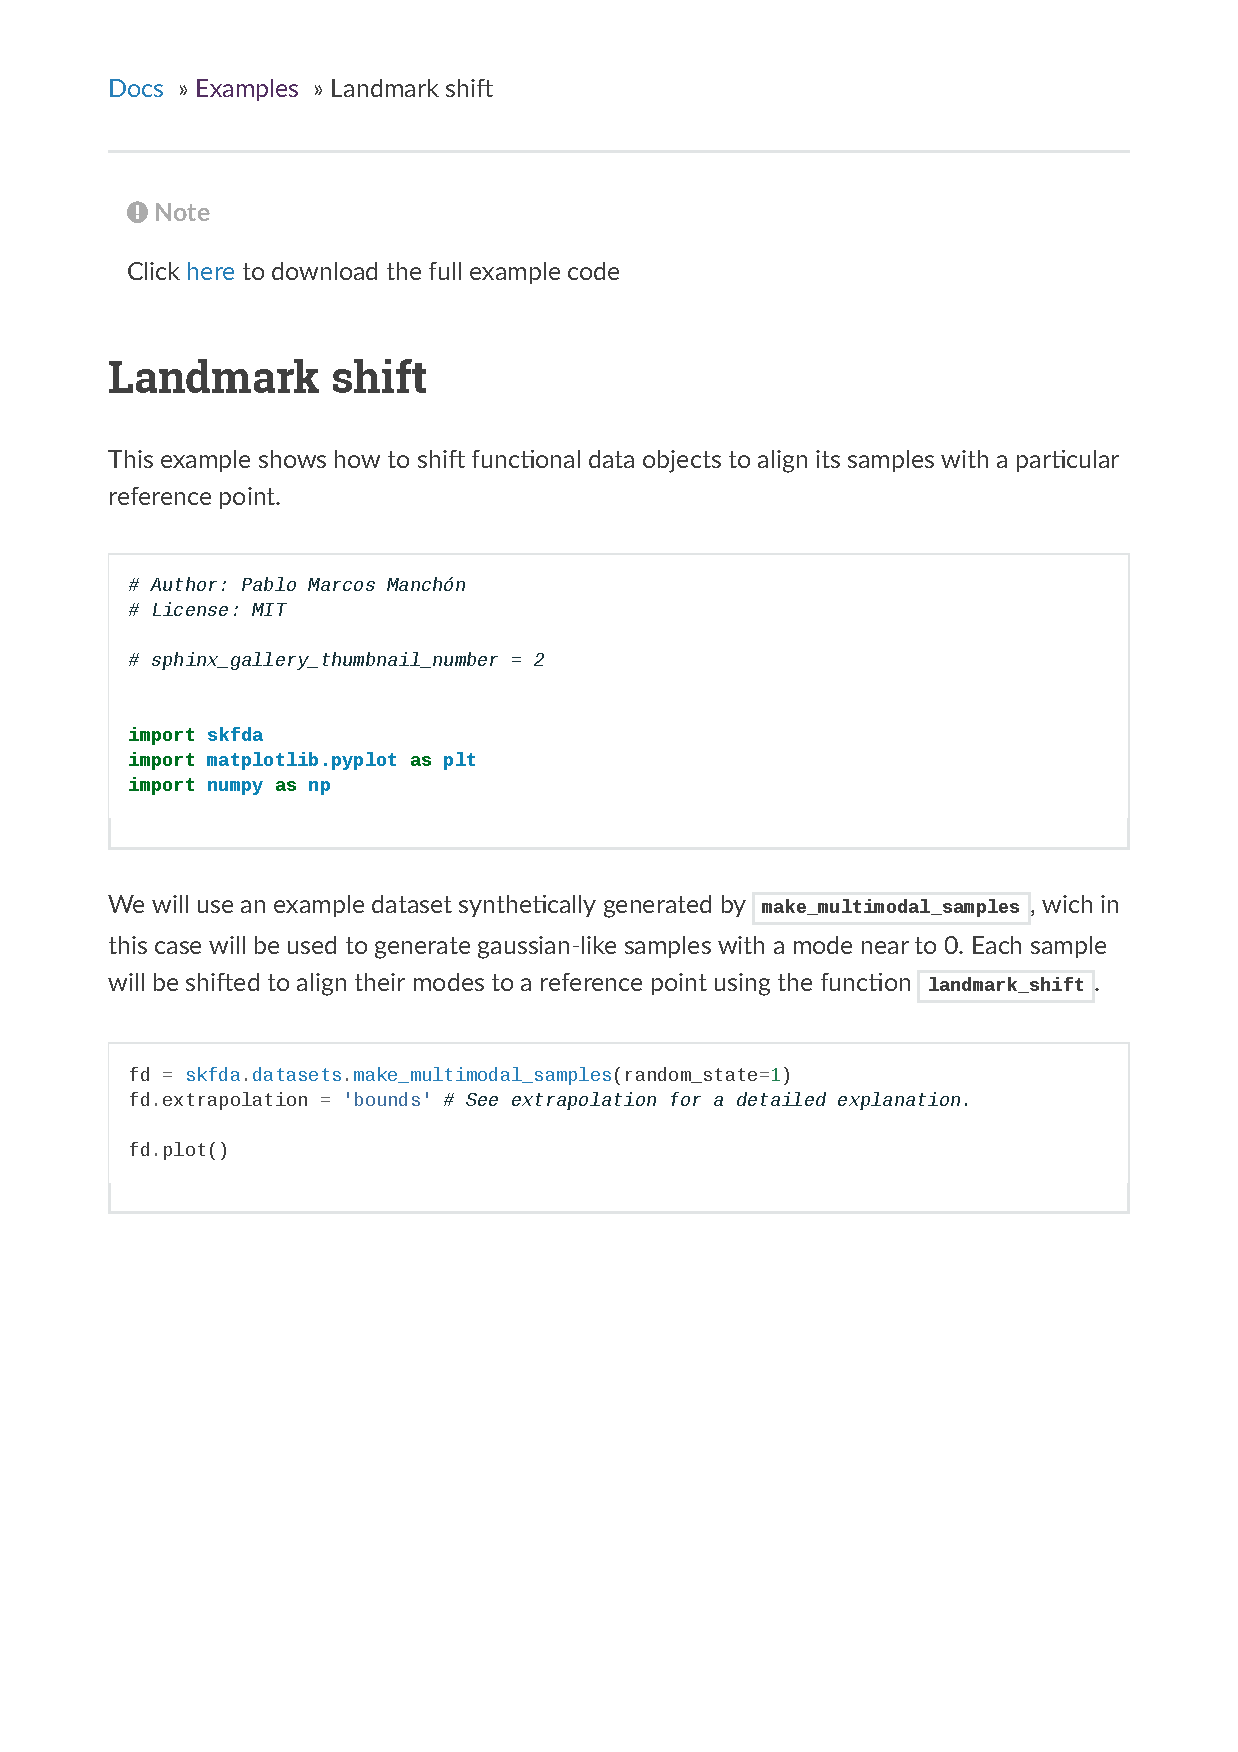
\includepdf[pages=-, nup=2x2]{notebooks-pdf/Landmark-shift}

%\section{Landmark registration\label{EX:LANDMARKREG}}

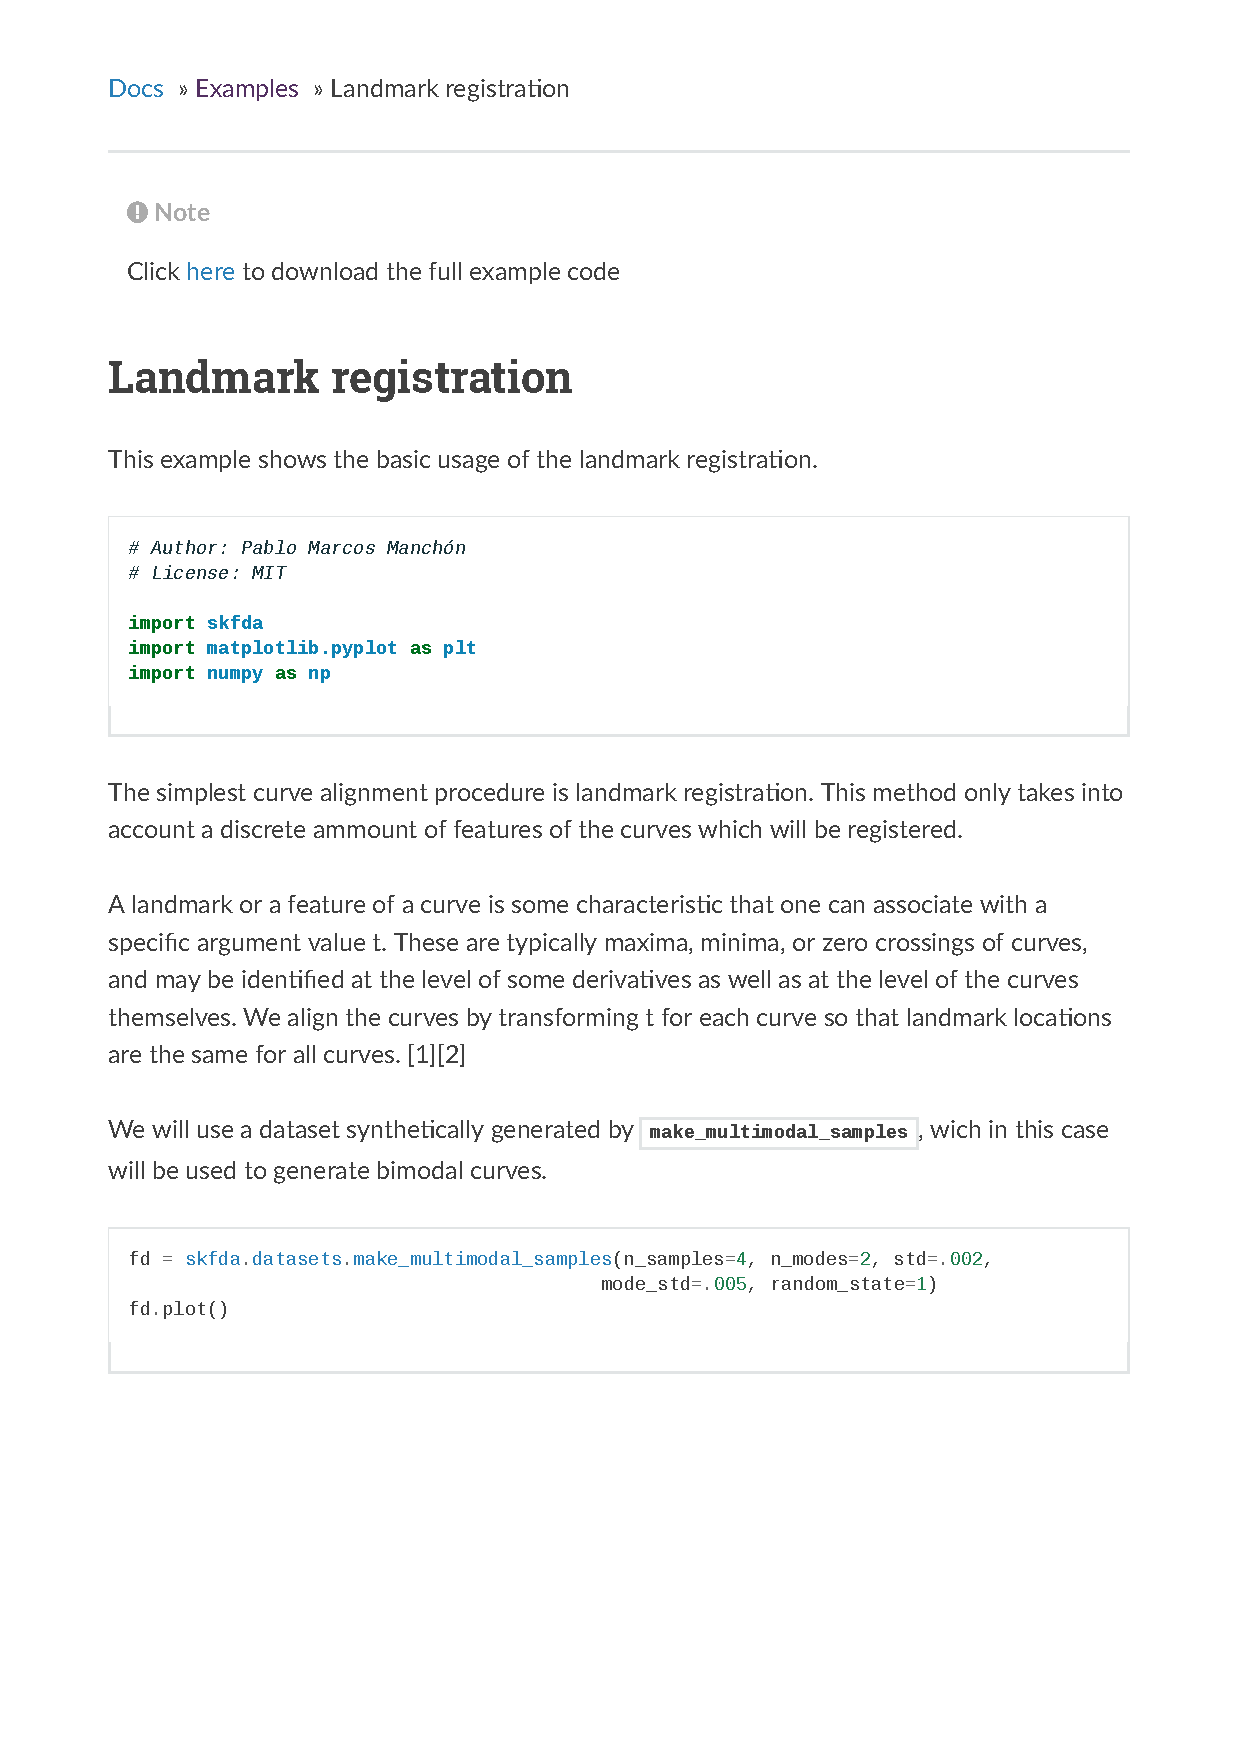
\includepdf[pages=-, nup=2x2]{notebooks-pdf/Landmark-registration}

%\section{Pairwise alignment\label{EX:PAIRWISE}}

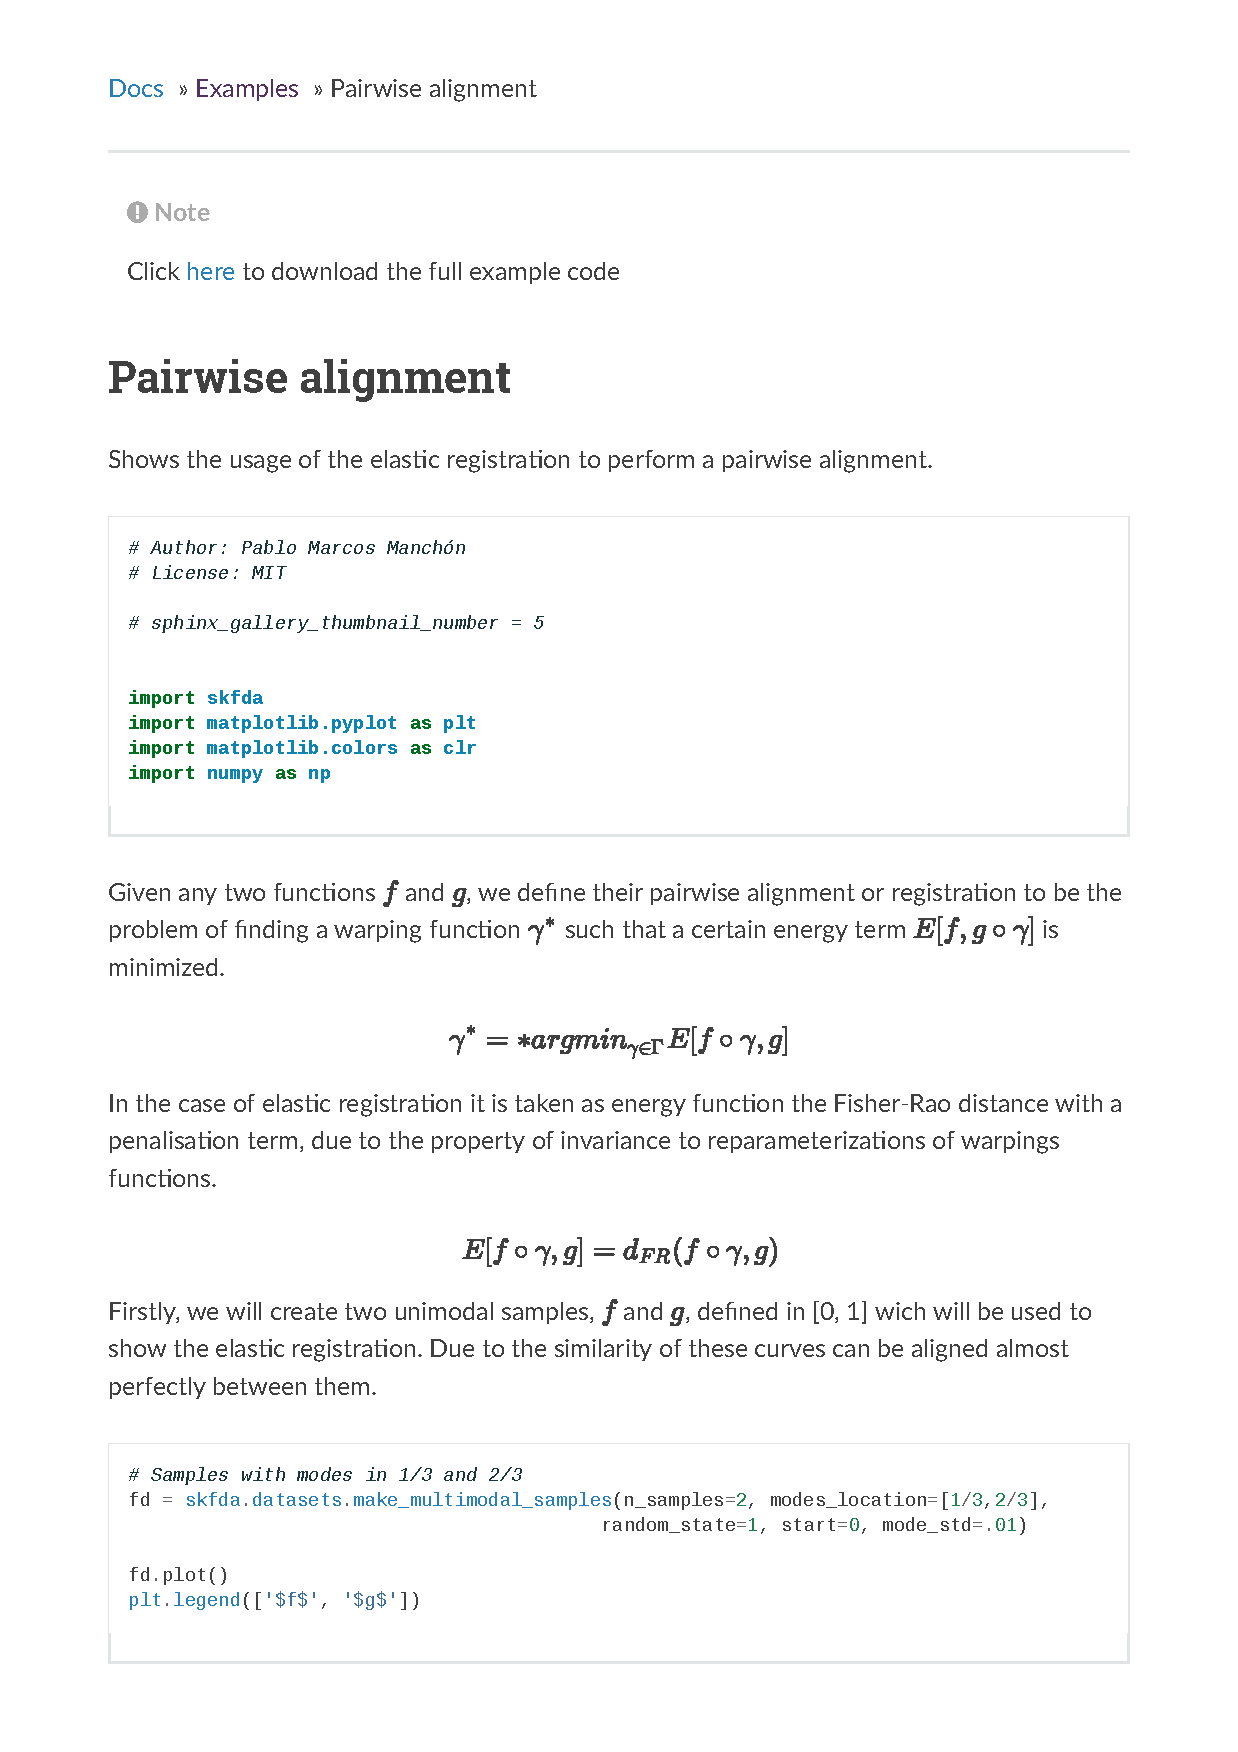
\includepdf[pages=-, nup=2x2]{notebooks-pdf/Pairwise-alignment}

%\section{Elastic registration\label{EX:ELASTIC}}

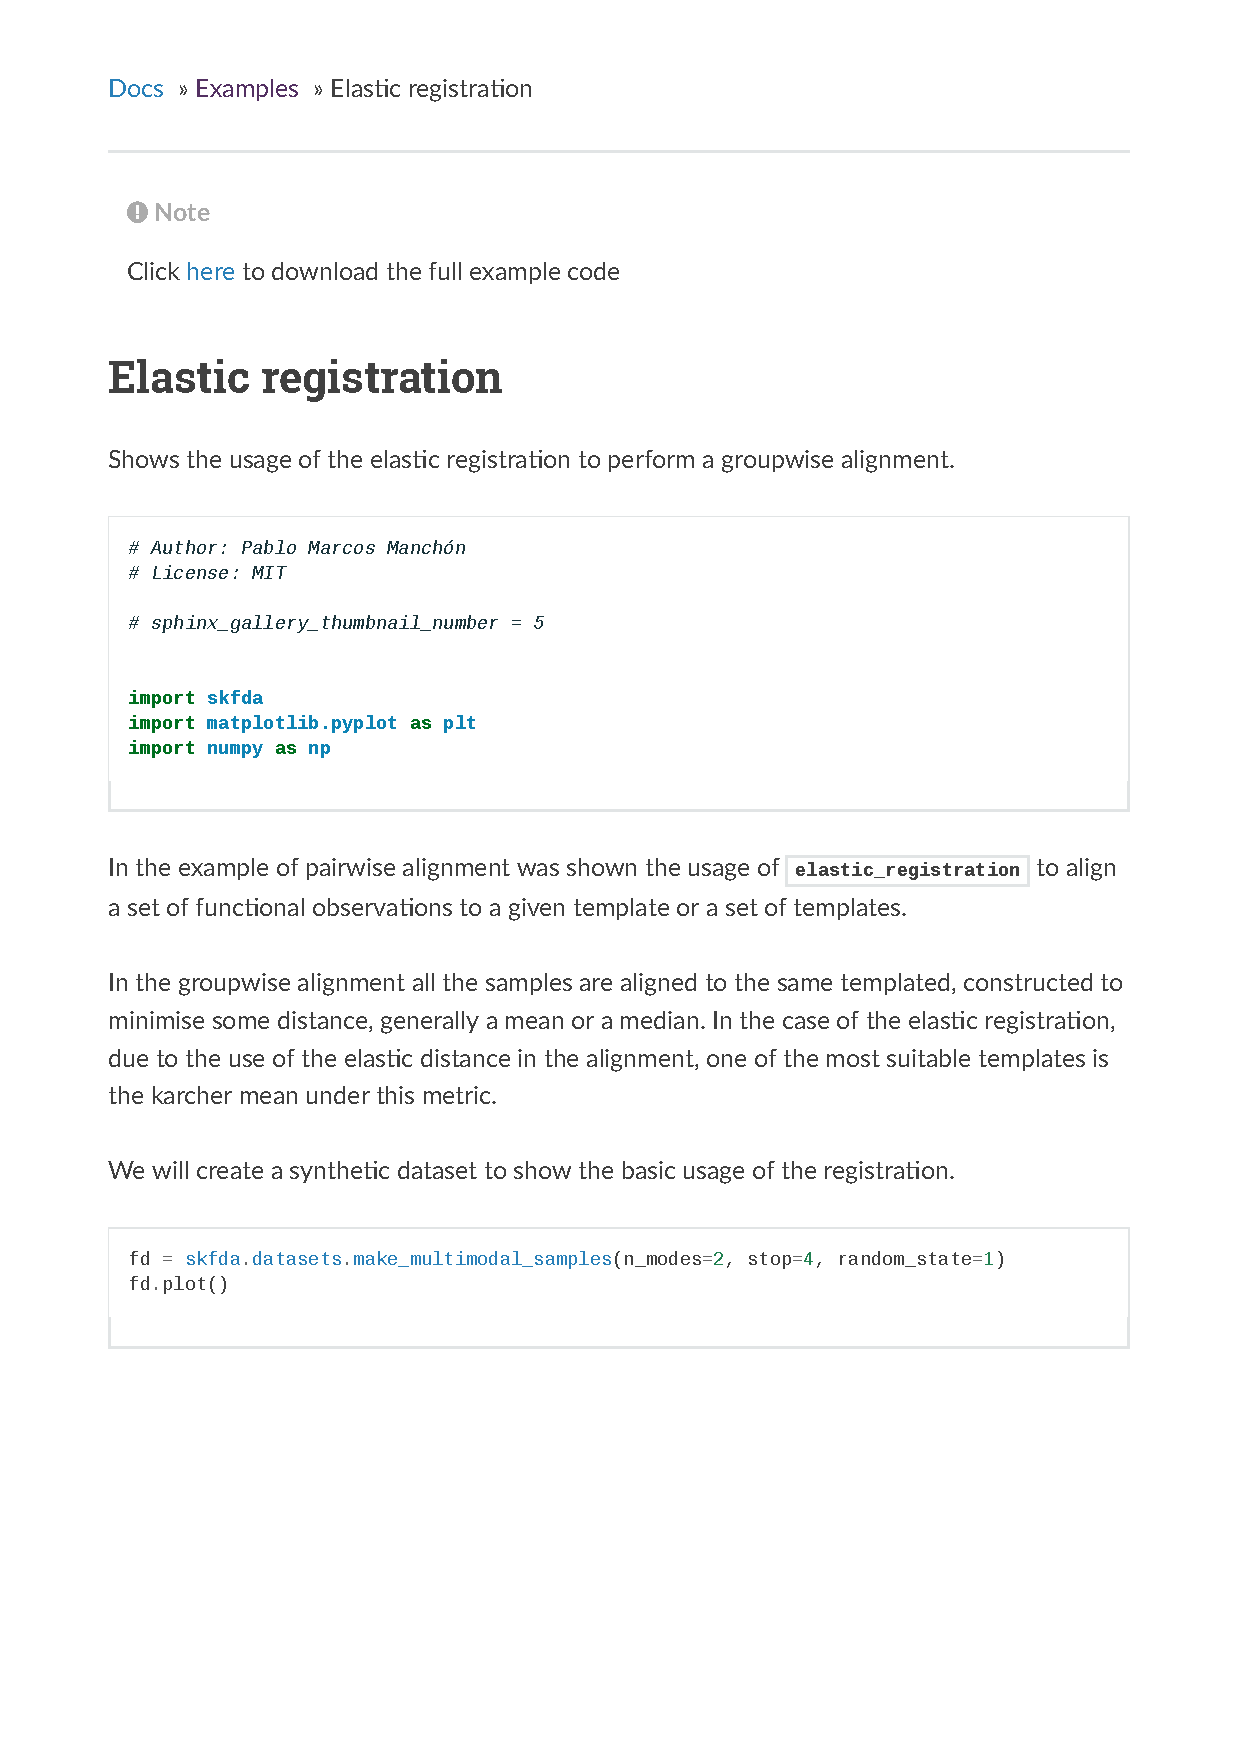
\includepdf[pages=-, nup=2x2]{notebooks-pdf/Elastic-registration}

%\section{K-nearest neighbors classification\label{EX:KNN}}

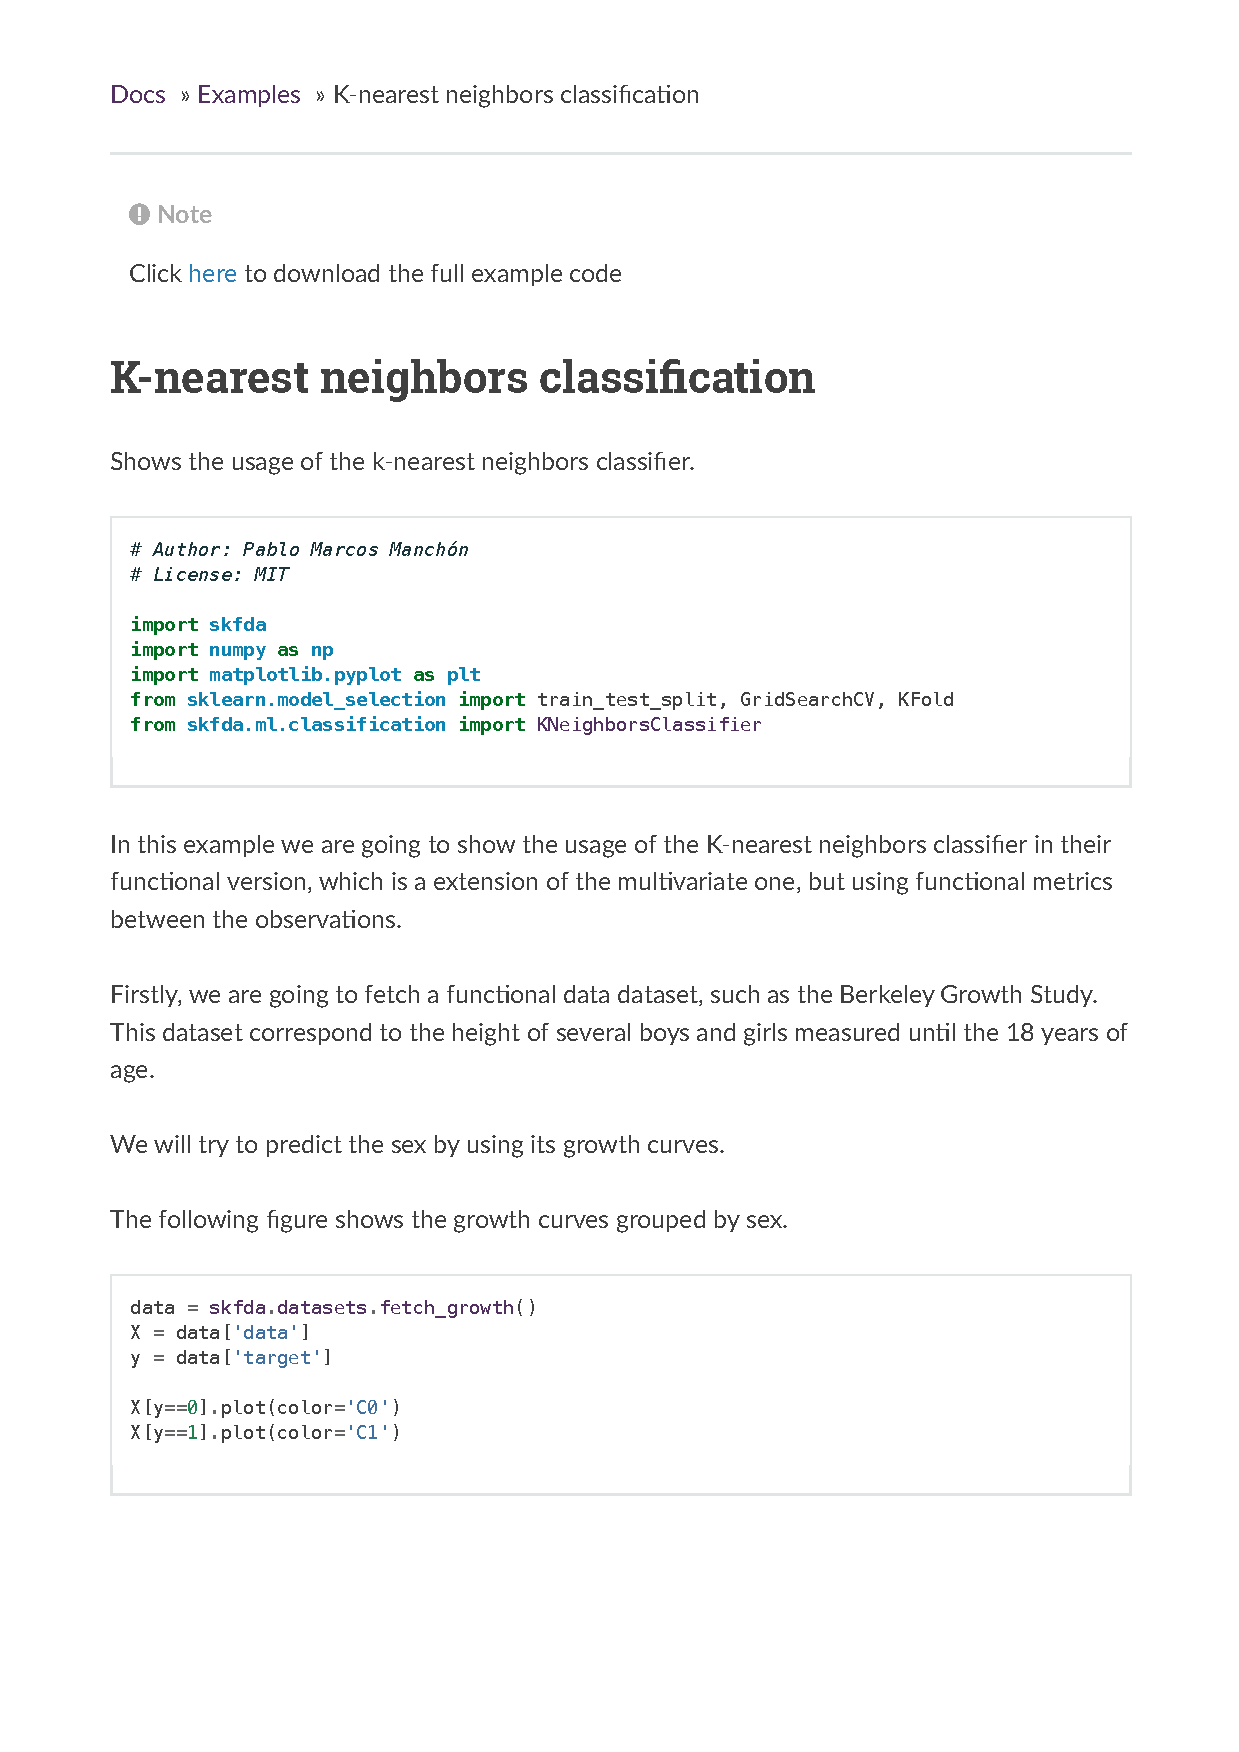
\includepdf[pages=-, nup=2x2]{notebooks-pdf/K-nearest-neighbors-classification}

%\section{Radius-NN classification\label{EX:RNN}}

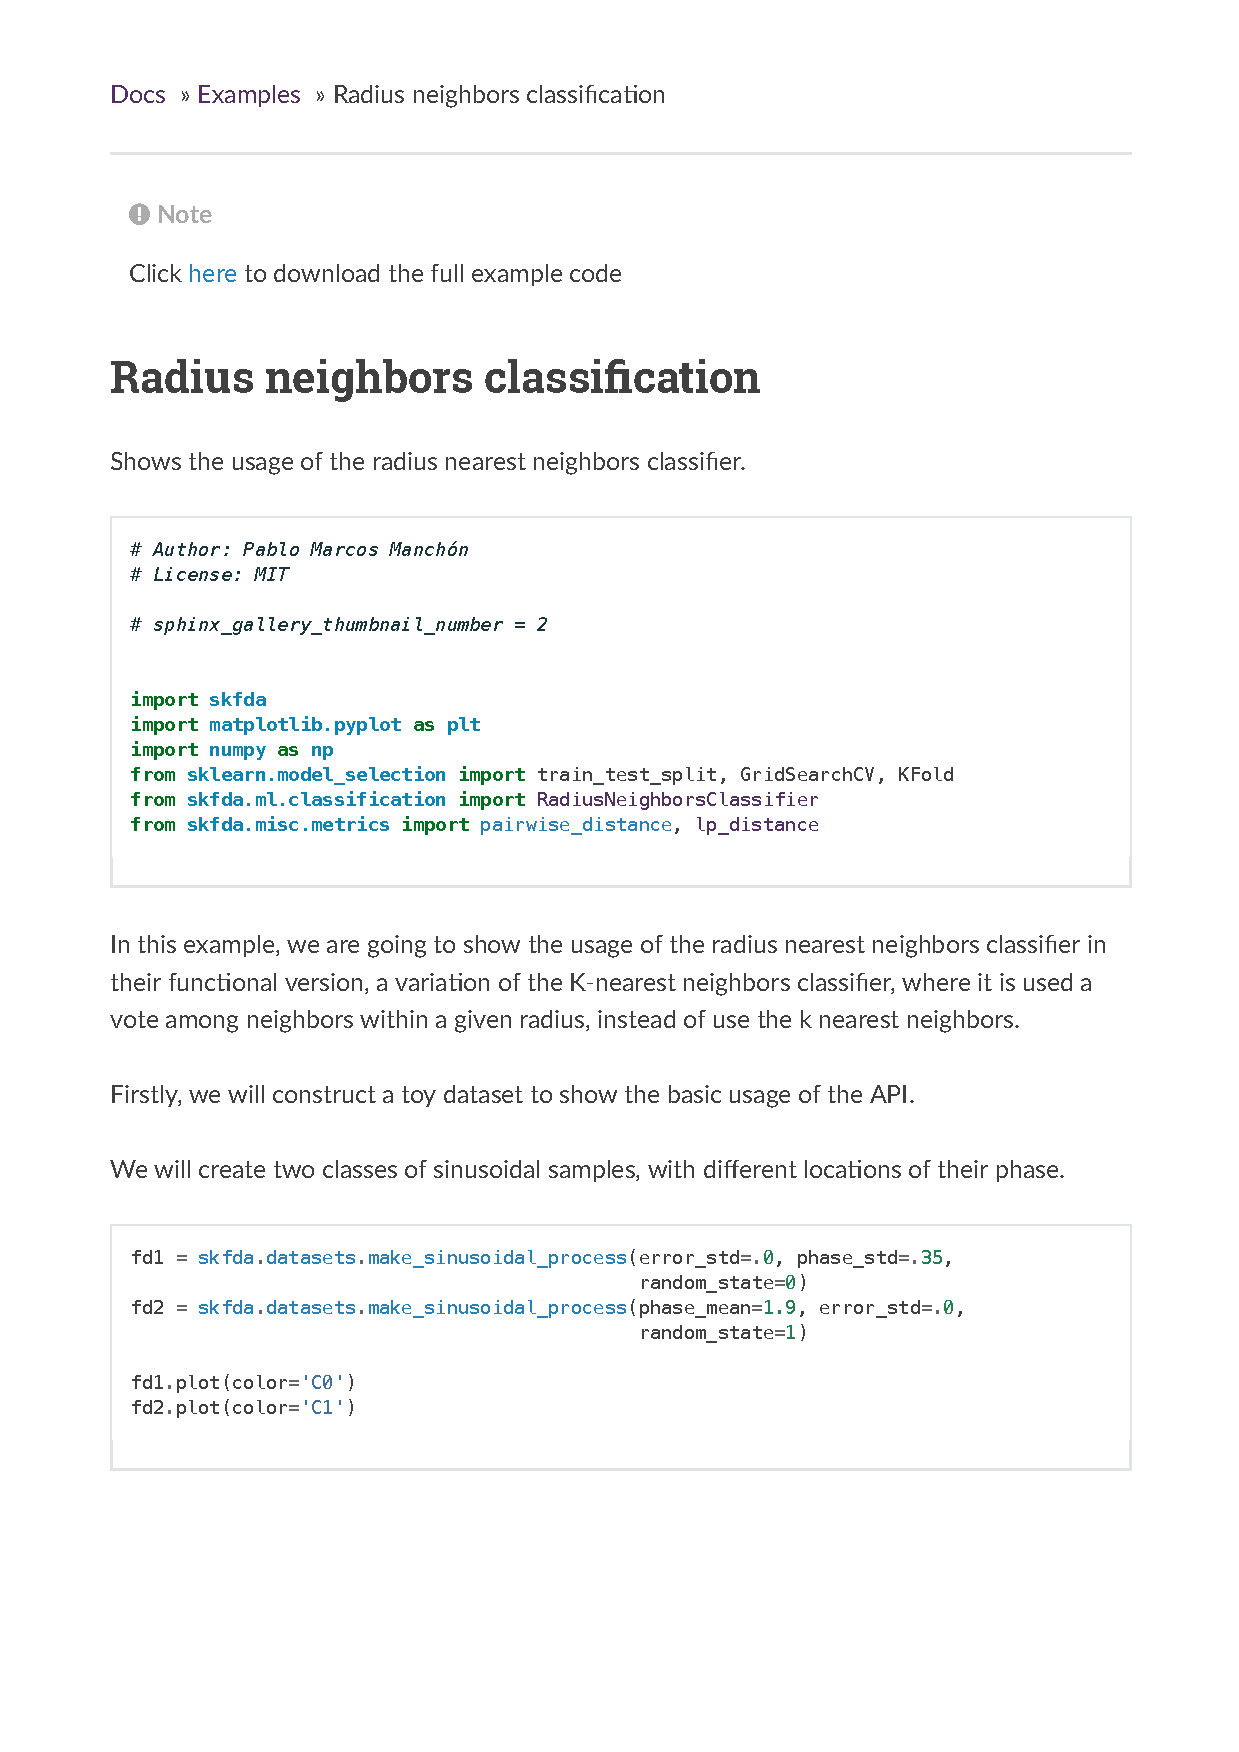
\includepdf[pages=-, nup=2x2]{notebooks-pdf/Radius-neighbors-classification}

%\section{Neighbors scalar regression\label{EX:SCALARREG}}

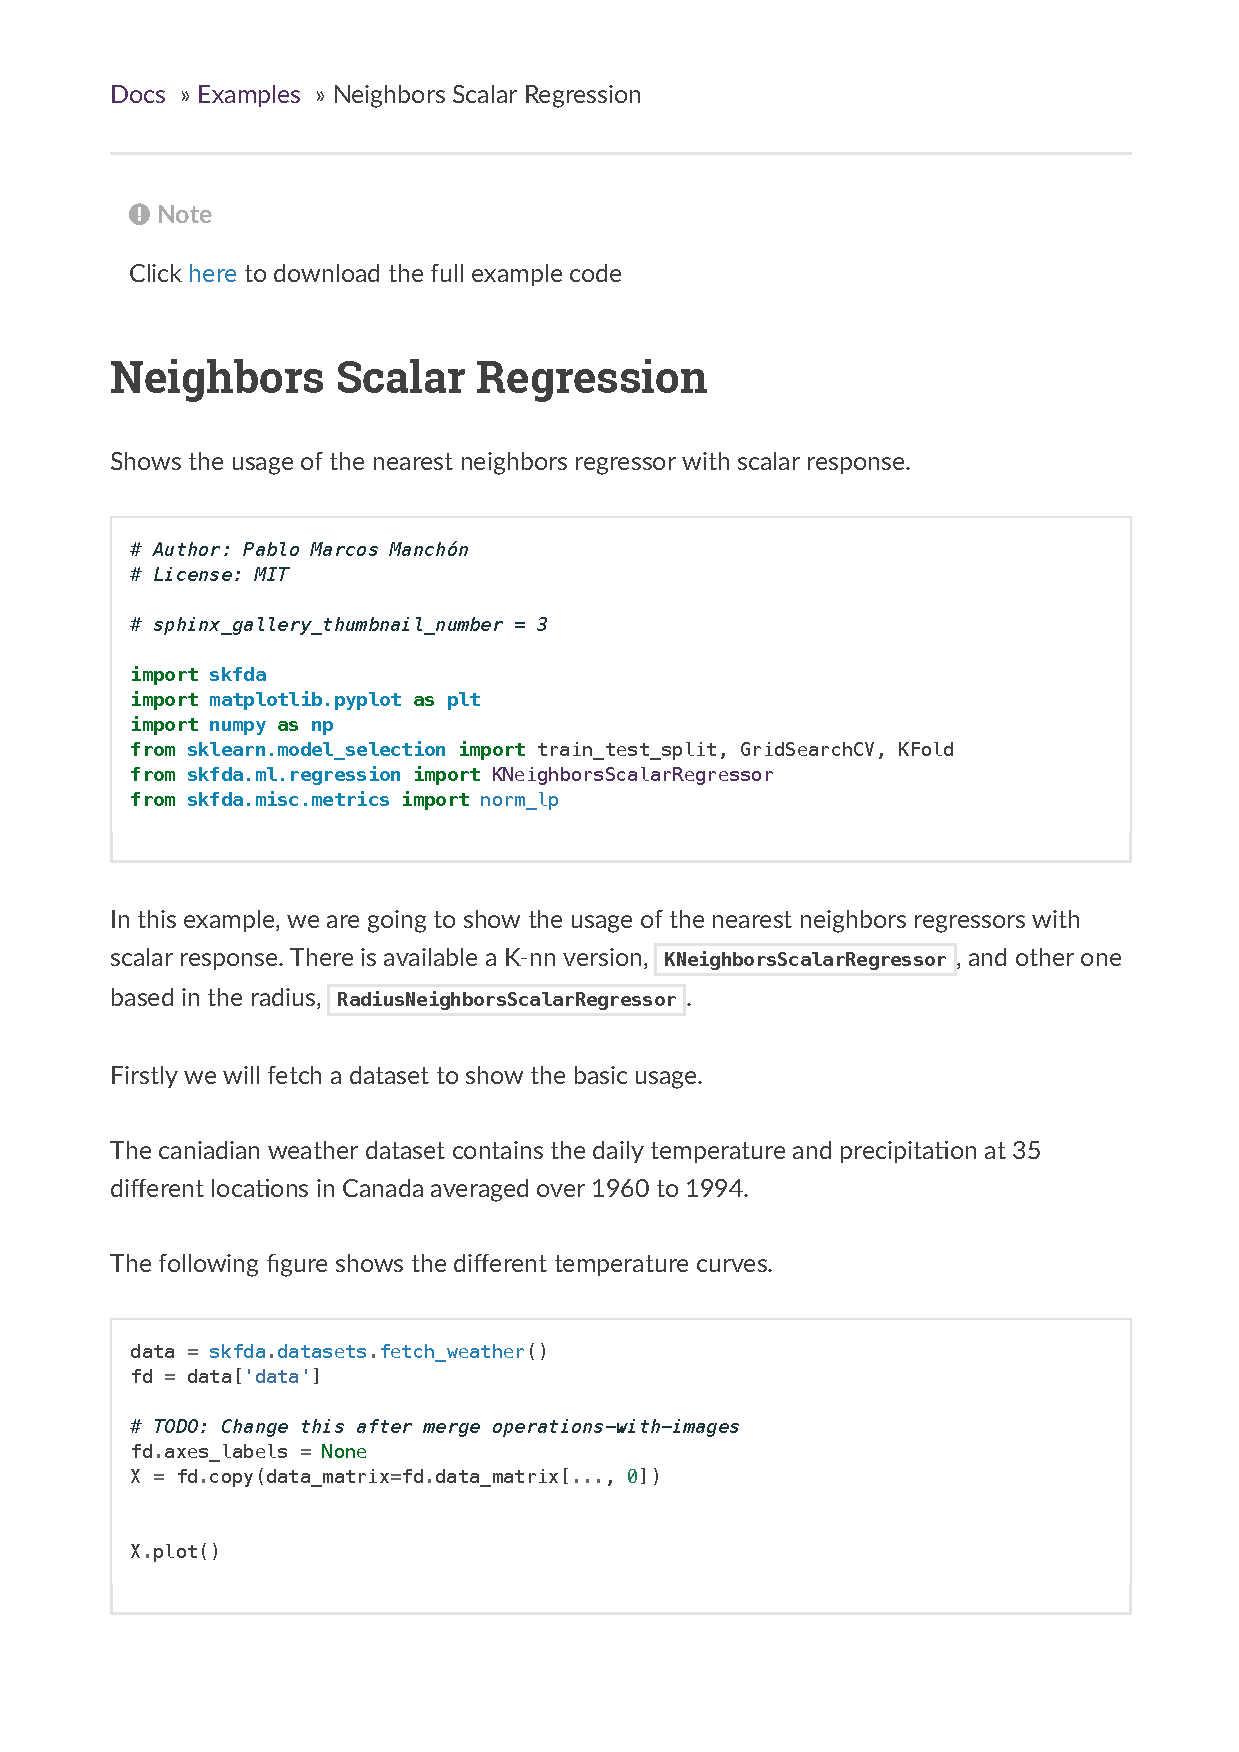
\includepdf[pages=-, nup=2x2]{notebooks-pdf/Neighbors-scalar-regression}
